%\documentclass[preprint]{sigplanconf}
\documentclass{article}
\usepackage[margin=1in]{geometry}

% The following \documentclass options may be useful:
%
% 10pt          To set in 10-point type instead of 9-point.
% 11pt          To set in 11-point type instead of 9-point.
% authoryear    To obtain author/year citation style instead of numeric.
%\usepackage{fontspec} % Doesn't work with LaTeX
\usepackage{graphicx}
\usepackage{amsmath}
\usepackage{color}
%\usepackage{multirow}
%\usepackage{sectsty}
%\usepackage[titles]{tocloft}
%\usepackage{sidecap}
\usepackage{multicol}

\title{Library-based fault tolerance for scientific applications}
\author{Sui Chen for EE7091 independent research, Fall 2012}
\begin{document}

\maketitle

%\conferenceinfo{WXYZ '05}{date, City.} 
%\copyrightyear{2005} 
%\copyrightdata{[to be supplied]} 

%\titlebanner{banner above paper title}        % These are ignored unless
%\preprintfooter{short description of paper}   % 'preprint' option specified.


%\subtitle{Subtitle Text, if any}

%\authorinfo{Name1}
%           {Affiliation1}
%           {Email1}
%\authorinfo{Name2\and Name3}
%           {Affiliation2/3}
 %          {Email2/3}

%\maketitle

%\begin{abstract}
%This is the text of the abstract.
%\end{abstract}

%\category{CR-number}{subcategory}{third-level}

%\terms
%Accuracy metric and Running time metric

%\keywords
%Resilience, High-performance computing, Algorithmic fault tolerance, Scientific libraries

This report documents the work based on the DSN 2012 poster (attached) spanning from the summer break to the end of this semester.

\section{Introduction}

As the size of HPC system grows to millions of processor cores and chip features shrink to a fraction of nanometers, HPC applications are increasingly threatened by transient hardware faults. Such faults can cause application aborts and performance degradation. More importantly, they may corrupt application results. As such, applications must be
made resilient to soft faults.

Such faults can be detected by running the application multiple
times and comparing the results. While simple and effective,
this approach is very inefficient. This inefficiency is
particularly important for Exascale systems, which will be
highly vulnerable to soft faults but will also be severely power-
constrained. This makes it necessary to develop alternative
techniques that leverage application semantics to provide
resilience at a lower cost.

We present a library-based approach to algorithmic
resilience where only the key application libraries are made
resilient and no protection is provided to the rest of the
application’s logic. By ensuring that the bulk of algorithmic
modifications is localized to libraries, where most application
time is spent, this approach balances developer effort against
performance and resilience to achieve high overall
productivity. We also explore various trade-offs that could be made in the choice of configurations for the fault tolerance parameters.


\section{Manifestation of errors}

As from the view of a user of supercomputers, errors would manifest themselves by:
\begin{itemize}
\item{Corrupting pointers/data structures, ensued by segmentation faults that terminate the application of other unexpected control flow changes.}
\item{Corrupting results that are used as input into subsequent routines, rendering the output of the application useless.}
\end{itemize}

Over-frequent termination of applications results in longer expected time to get acceptable results if the user had no choice but re-start the application over and over. Specially, this could be illustrated with the following Markov Model \ref{markovModel}.

\begin{figure}
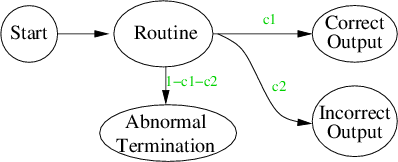
\includegraphics[width=6cm,natwidth=398,natheight=162]{routine_markov.png}
\caption{The Markov Model illustrating a numerical routine we're interested in. This routine, under the effects of soft errors, may abort and produce no results at all or it produce erroneous results or under some circumstances produce correct results. If the user keeps restart the application in case of error, the expected completion time of the routine could be computed as $T=(2-c)B+{{1-c} \over {c}} \cdot R$}
\label{markovModel}
\end{figure}

This model reveals the efficneicy concerns of fault-tolerance routines. The user is facing the choice of running multiple times the original application and running the fault-tolerant version of the application which is slower. The overhead of fault-tolerant routines are acceptable only when the fault-tolerant routines are capable of bringing down the \emph{expected} completion time to some acceptable level in comparison to running the original application multiple times.

\section{Library-Based Algorithmic Fault Tolerance}

Library-based algorithmic fault tolerance leverages the special properties of the computation routines used in those applications to provide cost-effective resilience. Because soft faults can corrupt arbitrary parts of the application's execution state, algorithmic fault error checkers could be very hard to implement to cover all possible vulnerabilities in practice, and even if it's possible, the amount of manual labor required would be prohibitively high. As such, to achieve the best balance between the costs of incorrect algorithm results, power use and development time, the most cost-effective approach would be to focus the algorithmic approach on application libraries, whose execution take up most of the CPU time. Libraries such as numerical solvers take up most of applications' execution time, therefore high resilience could be achieved at a low developer cost by focusing on implementing resilience on just those software components.

\section{Fault Injection}

Since the cause of soft errors could be complicated and it's hard to simulate them in an physically accurate way, we use error injection to simulate soft faults. We use a tool based on LLVM originally developed to evaluate the Relax framework \cite{deKruijf:2010:RAF:1816038.1816026} . It compiles the application (together with the library) into LLVM code, chooses random LLVM instructions during the application's execution and corrupts the results. As has been illustrated in the previous section, the errors manifest themselves by corrupting the outputs, or causing unexpected aberration in the control flow of the applications. For errors, to error magnitude is measured multiplicatively: if $x$ is the correct value and $x'$ is the erroneous one, error is measured as $|{x' \over x - 1}|$. This ratio is afterwards used in later sections to compute an \emph{accuracy metric}. The change in control flow may bring the application to a complete stop, requiring a restart, prolonging the expected time needed to get meaningful results. The time is taken into account in the \emph{running time metric}.

Errors are injected into the routines and the fault-tolerance code as well.

\begin{figure}
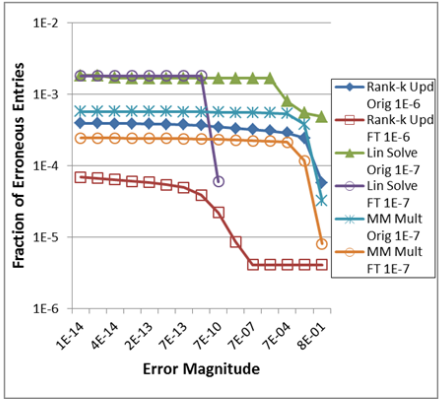
\includegraphics[width=6cm,natwidth=440,natheight=401]{vuln-gsl.png}
\caption{Error vulnerability of GSL routines. The figure shows the fraction of entries in the output matrix (the vertical axis) that have an error large than some magnitude (the horizontal axis). The fault-tolerance mechanism we have used here have reduced the occurances of errors of all magnitudes by one magnitude for routines Rank-K update and Matrix-matrix multication, and has removed the worst errors in the TRSV linear solver. This proves the fault-tolerant versions of the routines are effective.}
\label{vulnerabilityGSL}
\end{figure}

\subsection{List of fault injection applications}

We evaluate our library-based resilience approach by applying it to three applications.

\begin{itemize}
\item{Lasso: a parallel shrinkage and selection method for linear regression. It computes the equation $Ax=b$, where matrix $A$ and vector $b$ are known.}

\item{DRC: Digital Room Correction, a program used to generate correction filters for acoustic compensation of HiFi and audio system in general. It generates FIR correction filters, which can be used with a real time or offline convolver to provide correction.}

\item{Hattrick: An accurate N-Body integrator meant for high control over small systems, specifically meant for perturbing bodies.}

The three applications make intensive use of GSL (the GNU Scientific Library)'s linear algebra, FFT and differential equation solvers and therefore, they are ideal testbeds for our proposed fault-tolerance methods.

\end{itemize}

\section{Fault-Tolerant Routines}

As mentioned before, soft faults would cause corruption in outputs and change the application's control flow as well. Therefore countermeasures to each of these phenomenon is integrated into those fault-tolerance routines: algorithmic checkers and pointer/index replication. Construction of fault-tolerant routines consists of the following steps:

\begin{itemize}
\item{Identifying the most frequently used routines with GProf.}
\item{Constructing a wrapper function and set a signal handler to provide recovery ability upon segmentation faults.}
\item{Replicating critical data structures and pointers between library function calls.}
\item{In case of very high fault rate, replication of indices and pointers may provide further resilience to segmentation faults, albeit at a very high running time cost.}
\end{itemize}


\begin{figure}
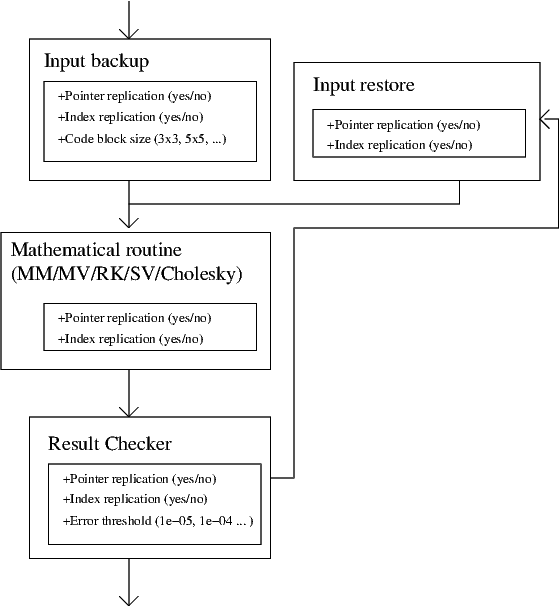
\includegraphics[width=8cm,natwidth=560,natheight=507]{flow.png}
\caption{Block diagram of fault-tolerant routines showing various parts: input backup, the original routine, result checkers and input restoration. The entire fault-tolerant routine is wrapped in a function call that has the same argument format as the original one, making it easy to be seamlessly integrated into applications.}
\label{faultRoutinesBlockDiagram}
\end{figure}


\section{Algorithmic Error Checkers}

For each routines used in above applications we develop corresponding fault checkers. As noted before, these checkers need be as fast as possible in order that the application could complete in a reasonable amount of time.

\begin{itemize}
\item{Checker for matrix-matrix multiplication:

Matrix-matrix multiplications are checked using a matrix vector multiplication, making use of this identity: $(A \cdot B) \cdot x = A \cdot (B \cdot x)$. Here x is a generated error-checking vector and $A$ and $B$ are inputs to the matrix-matrix multiplication. Time complexities of the original routine and the checker are $O(n^3)$ and $O(n^2)$ respectively.
}

\item{Checker for matrix-vector multiplication:

For matrix-vector multiplication $Ax=b$ , note that the sum of the elements in the result vector $b$ is equal to the dot product of the vector composed of column sums of $A$ and $x$. Time complexity of original routine is $O(n^2)$ multiplications and that of the checker is $O(n^2)$ additions.
}

\item{Checker for Symmetric Rank-K update:

Symmetric Rank-K update is a special case of matrix-matrix multiplication where only the upper/lower half of the output matrix is updated. By decomposing the upper/lower half of the output matrix as a series of sub-matrices (like the sub-cells in a quad tree), the checker takes $O(n^2 \cdot \log{n})$ time, while the original routine woudl take $O(n^3)$.
}

\item{Checker for Cholesky Decomposition:

By multiplying back the upper and lower halves, the checker takes as much time as a regular matrix-matrix multiplication would do. The original routine is an iterative one, but it generally runs longer than the checker.
}

\item{Checker for Fast Fourier Transform:

By using Parseval's Theorem, we can check the result of an FFT of width $n$ in $O(n)$ time. Time complexity of the original routine is $O(\log{n})$.
}

\end{itemize}

Those checkers can detect errors greater than a certain numeric threshold in those computations (determined by the user-defined error checker threshold). Once an error beyond the threshold has occurred, a re-calculation would be initiated.

In the following sections we would show that the error tolerance could not be arbitrarily small in order to be helpful in providing fault-tolerance when we take into account the checker itself may be unreliable since it's also vulnerable to soft errors.

\subsection{Picking an Arithmetic Error Detection Threshold}

Although checkers are faster than the routines they protect, the unreliability of those checkers and the ensuing ``false alarms'' might trigger redundant re-calculations that are unnecessary, causing the application to run for much longer. This is espqcially true with an overly small error detection threshold. On the other hand, an overly loose detection threshold may fail to detect data corruption in output files. The results would be discussed in the results section.

\section{Segmentation Fault Handlers}

Modern operating systems provide convenient means of protecting segmentation faults. A bombination of \texttt{siglongjmp} and \texttt{sigsetjmp} are used to recover from segmentation faults. The overhead of this API call is having to copy the processor state into memory, therefore installing them between computation-intensive method calls adds to neglible performance degradation.

\section{Input Data Protection}

Considering the fact that input data may be damaged, we need a fast yet simple mechanism with which we can easily identify and fix errors in the input. We have implemented a block-checksum-based data correction mechanism. By treating the input array as a matrix and comparing row sums and column sums of the submatrices of that matrix, we are able to detect the existence of errors and fix a fraction of the errors. The protection mechanism has the following parameters:

\begin{itemize}
\item{\texttt{N}, the size of the error correcting sum block.}
\item{\texttt{ECC\_ECC}, whether or not the error correcting code itself should be corrected.}
\end{itemize}

This mechanism is able to correct up to $1/{n^2}$ of the elements in the input array.

\section{Pointer and Index Replication}

The third application Hattrick uses a high-accuracy ODE solver that is capable of estimating errors and detecting and reducing errors to a certain level adaptively. Therefore we would only focus on the application's vulnerability to pointer and index corruptions. Replicating critical variables (pointers and indices) and leveraging Byzantine fault tolerance and correcting those pointers and indices during run-time would raise the applications' resistence to soft errors.

In order to determine a replication strategy we have to determine which variables to replicate and how many replicas to use for replicating them. The following two subsections would be focused on these problems.

\subsection{Determining which variables to replicate}

\begin{center}
\begin{verbatim}
1   for(i=0; i<M; i++) {
2     for(j=0; j<P; j++) {
3       double temp = 0;
4       for(k=0; k<N; k++) {
5         int idx_a = IX_A(i, k);
6         int idx_b = IX_B(k, j);
7         double elem_a = A[idx_a];
8         double elem_b = B[idx_b];
9         temp = temp + elem_a * elem_b;
10      {
11      int idx_c = IX_C(i, j);
12      C[idx_c] = temp;
13  }}
\end{verbatim}
\end{center}

And, suppose we have the following configurations for replication when M, N and P are 100.

\begin{figure}[h!]
\begin{center}
\begin{tabular}{|p{2.3cm}|p{8cm}|}
\hline
%\multicolumn{2}{|l|}{Configuration and pr}\\
Configuration & Protection applied \\
\hline
Baseline & without any protection for indices or pointers \\
Conf I-1 & protect indices j and k in innermost loop (line 4)\\
Conf I-2 & protect index j in second innermost loop (line 2); protect k in innermost loop(line 4) \\
Conf I-3 & protect index k in innermost loop (line 4)\\
Conf I-4 & protect indices i in outermost loop (line 1), j in second innermost loop, k in innermost loop \\
Conf P-1 & protect pointers A and B in innermost loop \\
Conf P-2 & protect pointers A and B in second innermost loop \\
Conf IP-1 & Conf I-4 plus Conf P-2 \\
\hline
\end{tabular}
\end{center}
\caption{Configurations applied upon the previous code snippet.}
\label{fig:confsAndProtections}
\end{figure}

\begin{figure}[h!]
\begin{center}
\begin{tabular}{|p{2.3cm}p{1cm}p{1cm}p{1cm}p{2.2cm}|}
\hline
Configuration & \multicolumn{3}{c}{Completion rate at errors per run} & Running time\\
\hline
Baseline & 0.86 & 0.60 & 0.00 & 1x \\
Conf I-1 & 0.92 & 0.60 & 0.00 & 1.87x \\
Conf I-2 & 0.92 & 0.67 & 0.00 & 1.47x \\
Conf I-3 & 0.92 & 0.65 & 0.00 & 1.14x \\
Conf I-4 & 0.91 & 0.61 & 0.01 & 1.47x \\
Conf P-1 & 0.97 & 0.65 & 0.03 & 2.04x \\
Conf P-2 & 0.95 & 0.69 & 0.05 & 1.28x \\
Conf IP-1 & 0.94 & 0.73 & 0.05 & 1.74x \\
\hline
\end{tabular}
\end{center}
\caption{Effectiveness of the pointer/indices replications configurations listed above}
\label{fig:effectivenesses}
\end{figure}

From the results (Figures \ref{fig:confsAndProtections}, \ref{fig:effectivenesses} on page \pageref{fig:confsAndProtections} and \pageref{fig:effectivenesses}) we see the best resilience is obtained when we protect both pointers and indices and that indices should be protected in the same loop level as where they were declared, so that their values are read and overwritten no more often than their values are incremented by the for loop. 

\subsection{Finding the Best Replication Strategy}

In some circumstances we don't have much choice over where to protect those pointers or indices, for example:

\begin{center} \begin{verbatim}
1  double *in, *out;
2  for(i=0; i<M; i++) {
3     complicated_computation1(in, out);
4     complicated_computation2(in, out);
5     complicated_computation3(in, out);
6  }
\end{verbatim} \end{center}

In this scenario, the only place (in this source code) we can protect the values of pointers in and out would be between lines 2, 3, 4, 5 and 6. To make protection more effective, we would use more replicas instead of updating the replicas more often. As more replicas are used, one must be aware that when each replica is cold-loaded into the CPU's register file a load instruction is executed, and it is a possibly vulnerable instruction. Therefore, re-using replicas should reduce the vulnerabilities brought by load instructions. However the longer replicas are kept in memory the more likely the the replicas would also be corrupted. To find the number of replicas, we have tried different numbers at which the variables are replicated, as well as how many pointers we cover. The code experimented was the RK4 integrator used in Hattrick and the results are listed in Figure \ref{fig:greenMtx}.

\begin{figure}[h!]
\begin{center}
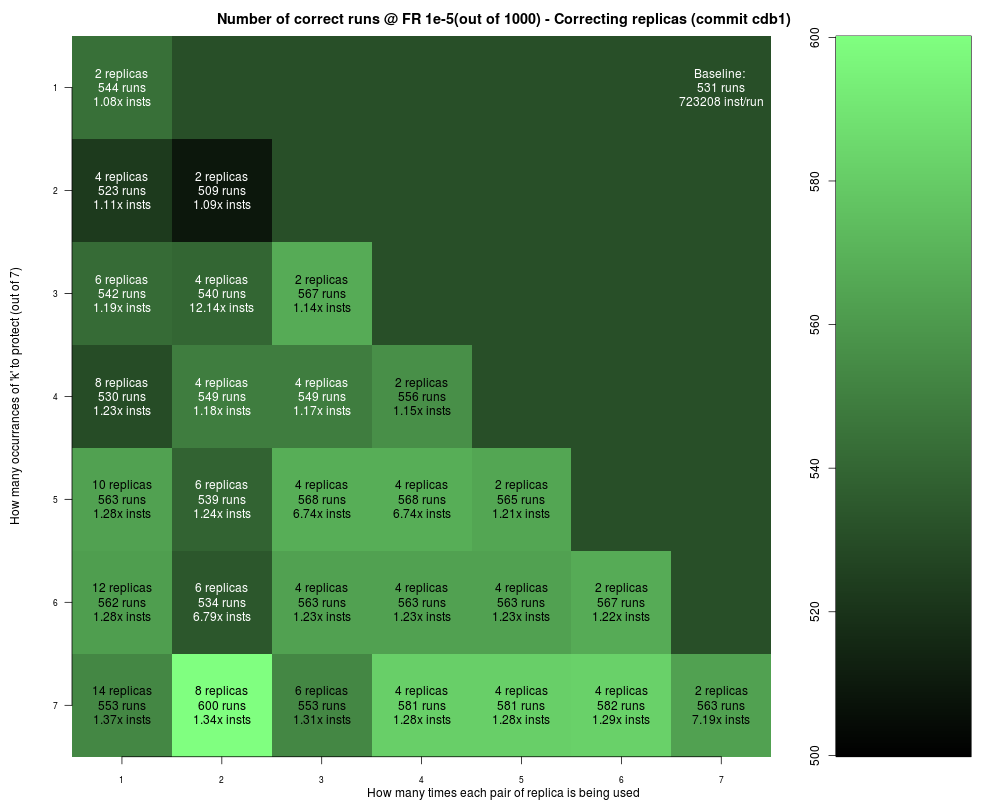
\includegraphics[width=10cm,natwidth=1000,natheight=800]{n_replica_correct_runs_cdb1.png}
\end{center}
\caption{Effectiveness of pointer and index replication in RK4 integrator. The X axis is how many times each pair of replica is used and the Y axis is how many occurrances of a loop variable to protect. Obviously, we have the best resilience when all occurrances are protected. The interesting discovery is that using each replica twice instead of once has the best resilience. The color of the cells indicate the relative resilience: the brighter, the more resilient.}
\label{fig:greenMtx}
\end{figure}

\section{The metrics}

We derive the metrics for expected running time and accuracy of outputs. These metrics make it possible to meaningfully compare results of the same application across different input files with different failure-free execution times. The combined metric is a product of both metrics and therefore would reflect the tradeoff between accuracy and expected running time.

The metrics are computed on each run of an application; the metrics require data collected from both faulty runs and fault-free runs.

\subsection{Accuracy metric}

The correctness metric is defined as:

\[
m_{accu} = \left \{
	\begin{array} {l l}
	10 & \: \text{if RMSD is less than $1e^{-10}$} \\
	-\log(RMSD) & \: \text{otherwise} \\
	\end{array} \right.
\]

The correctness metric makes it possible to make reasonable comparisons between
different configurations (i.e. fault-tolerance techniques used, input size, fault rate)
of the same application. The accuracy metric is bounded to avoid having to take the
logarithm of zero.

\subsection{Running time metric}

\[
m_{runt} = \left \{
	\begin{array} {l l}
	3-\log_2{\frac{RT_{faulty}}{RT_{faultfree}}} & \: \text{if $\frac{RT_{faulty}}{RT_{faultfree}}$ < 8} \\
	0 & \: \text{otherwise} \\
	\end{array} \right.
\]

The running time metric is capped at 0 to reflect our consideration that one run that takes too much time to complete would be much less preferrable for the user. An unreasonably long running time might be caused by an overly strict error detection threshold for the fault rate under which the experiment is executed. Therefore the user might wish to loosen the error detection threshold in exchange for faster execution.

\subsection{Combined metric}

The combined metric is simply a product of the two aforementioned metrics.

\[
metric = m_{accu} \cdot m_{runt}
\]

It would reflect the overall result of tradeoffs between running speed and accuracy: The user may choose to trade some running speed for accuracy and result in a better performance of the faulty application.

\section{Fault Tolerance Experiment Results}

\subsection{Results of LASSO}

We are generating input data for Lasso program. Data size varied from 10x to 100x, and we are injecting errors into Lasso at different fault rates. Figure \ref{fig:lassoTable} is the result of representative runs of Lasso, and figure \ref{fig:chickGraphLasso} has an overview of the influence of different algorithmic checker thresholds.

\begin{figure} \begin{center} \begin{tabular}{p{2.5cm}p{2cm}p{2cm}p{2cm}p{2.5cm}p{2.5cm}}
\hline
Configuration and fault rate & SegFault Rate & Errors handled per run & RMSD per run & Measured Running Time & Expected Running Time \\
\hline
\multicolumn{6}{l}{Input 1 (Size = 40x500)} \\
Baseline 1e-8 & 11\%  &         & 1.13e-06 & 1.339s & 1.504s \\
FT 1e-8       & 0\%   & 1.49    & 3.7e-07  & 1.617s & 1.617s \\
Baseline 1e-7 & 76\%  &         & 5.85e-4  & 1.343s & 5.595s \\
FT 1e-7       & 15\%  & 14.29   & 6.44e-5  & 1.630s & 1.630s \\
Baseline 1e-6 & 100\% &         &          &        & Infinity \\
FT 1e-6       & 95\%  & 224.2   & 3.48e-5  & 1.915s & 38.3s  \\
\hline
\multicolumn{6}{l}{Input 2 (Size = 400x500)} \\
Baseline 1e-9 & 23\%  &         & 9.06e-5  & 3.947s & 5.126s \\
FT 1e-9       & 2\%   & 3.21    & 2.01e-5  & 7.623s & 7.779s \\
Baseline 1e-8 & 96\%  &         & 6.5e-4   & 3.928s & 98.2s  \\
FT 1e-8       & 45\%  & 59.89   & 4.5e-3   & 14.67s & 26.67s \\
\hline
\multicolumn{6}{l}{Input 3 (Size = 4000x500)} \\
Baseline 1e-11 & 32\% &         & 3.36e-6  & 28.92s & 42.53s \\
FT 1e-11      & 0\%   & 3.4     & 3.61e-6  & 62.6s  & 62.6s  \\
Baseline 1e-10 & 62\% &         & 6.56e-7  & 28.92s & 76.10s \\
FT 1e-10      & 0\%   & 7.1     & 1.64e-6  & 71.56s & 71.56s \\
Baseline 1e-9 & 80\%  &         & 2.88e-5  & 28.92s & 144.6s \\
FT 1e-9       & 20\%  & 36.8    & 5.83e-6  & 159.07s& 198.8s \\
\hline

\end{tabular}
\caption{Raw results of epresentative runs of Lasso}
\label{fig:lassoTable}
\end{center}
\end{figure}

\begin{figure}[h!]
\begin{center}
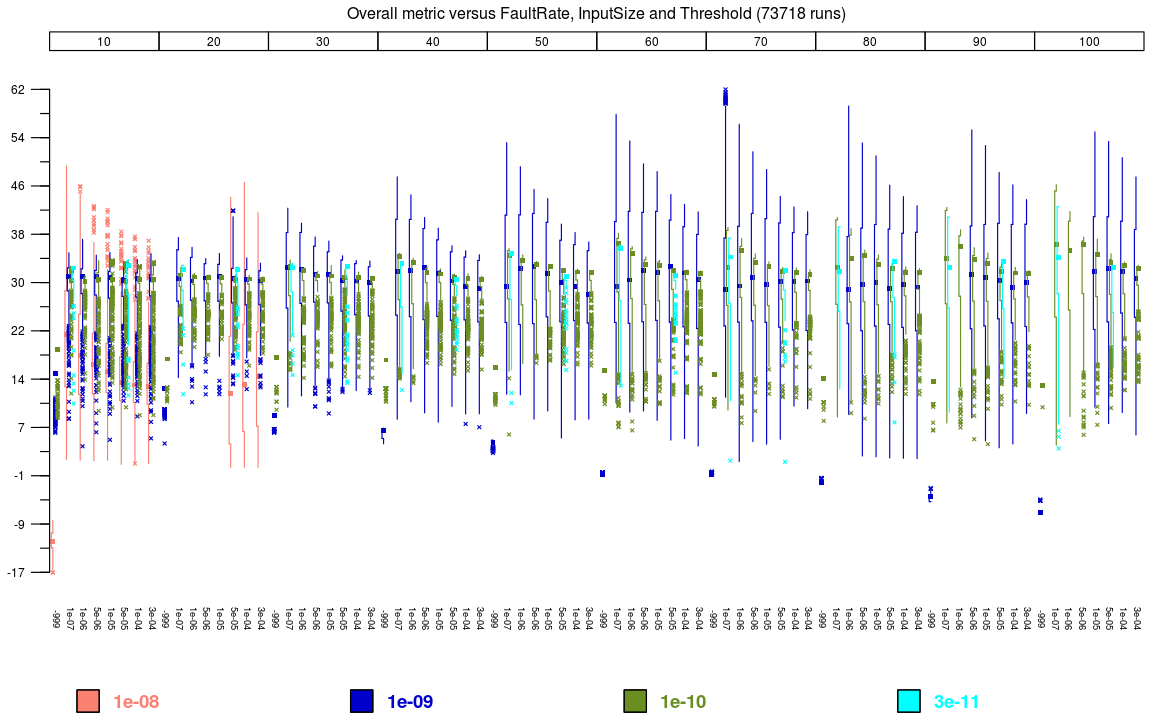
\includegraphics[width=16cm,natwidth=1156,natheight=725]{OverallMetric_Lasso_Boxplot.png}
\end{center}
\caption{Visualization of overall metrics of 73718 runs of Lasso throuout 256 different configurations. The facets correspond to different input sizes. The X and Y axes inside one facet correspond to different error checker thresholds and the overall metrics.}
\end{figure}

According to figure \ref{fig:lassoTable} For small inputs the fault-tolerant version of Lasso redcued segmentation fault rate and also reduced the expected completion time. For larger inputs, the fault tolerant version has an estimated running time on par with the non-fault-tolerant counterparts, but has less erroneous results, especially when the error rate is large.

\subsection{Results of DRC}

\begin{figure}[h!]
 \begin{center} \begin{tabular}{p{2.5cm}p{2cm}p{2cm}p{2.5cm}p{2.5cm}p{2.5cm}}

\hline
Configuration & SegFault Rate & Errors handled per run & RMSD per run & Measured Running Time & Estimated Running Time\\
\hline
Baseline 1e-11 & 66\% &         & 1.98e-4 & 26.51s & 77.97s \\
FT 1e-11       & 4\%  & 3       & 3.61e-6 & 35.54s & 37.02s \\
Baseline 1e-10 & 68\% &         & 6.56e-7 & 26.51s & 82.84s \\
FT 1e-10       & 15\% & 30      & 1.64e-6 & 37.65s & 44.29s \\
\hline
\end{tabular} 
\end{center} 

\end{figure}

\begin{figure}[h!]
\begin{center}
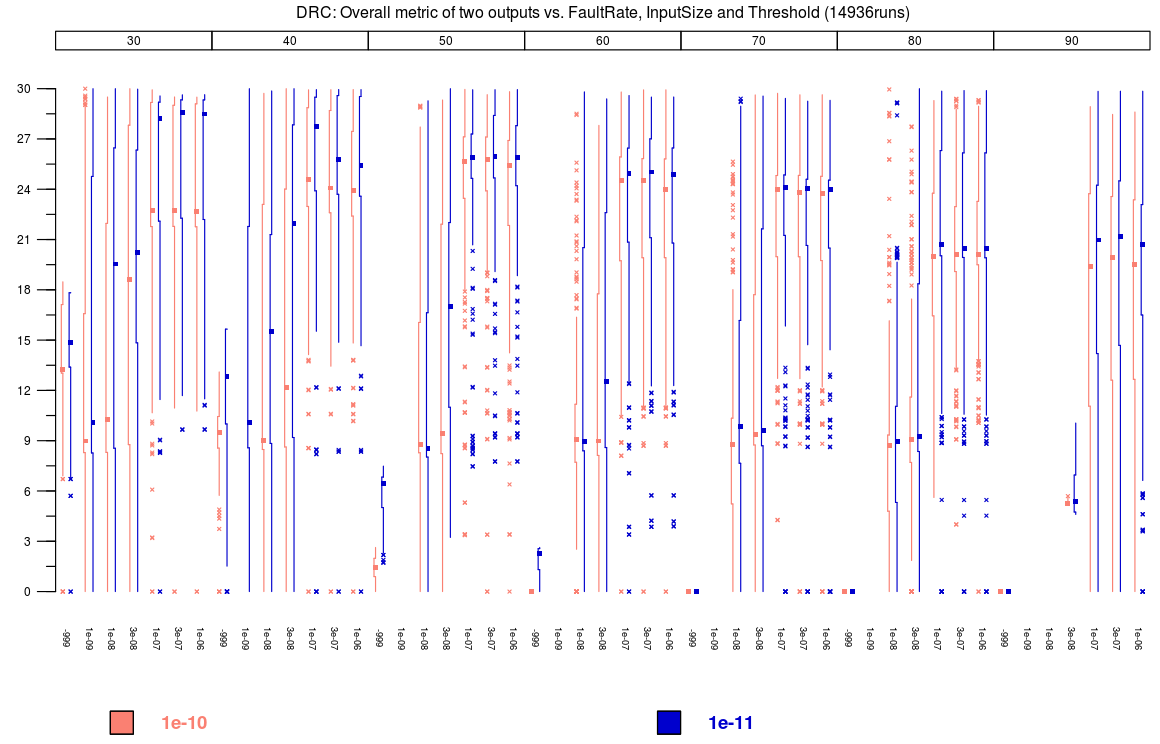
\includegraphics[width=16cm,natwidth=1160,natheight=744]{Overall_Metric_DRC.png}
\end{center}
\caption{Visualization of overall metrics of 14936 runs of DRC throughout 95 different configurations. The facets correspond to different input sizes. The X and Y axes inside one facet correspond to different error checker thresholds and the overall metrics.}
\end{figure}

From the results we could see our fault tolerance methods are both effective at reducing errors in output and reducing estimated running time. From the overall visualization we see the best choice of error checker threshold should be 1e-07. The optimal threshold is 1 magnitude smaller than that of Lasso due to the different characteristics of the routines used in both applications, the FFT and linear algebra.

\subsection{Results of Hattrick}

(Work still in progress)

\section{Estimation of running time under low error rates}

The results from previous sections have shown our resilience techniques are capable of protecting applications at a high error rate, when both the routines and the error checkers are vulnerable. As it's estimating runnning times for lower error rates may be inefficient and would require many runs, we propose using a Markov model to predict them.

Estimated completion time is computed in this way:

\[
T=(2-c) B + \frac{1-c}{c} \cdot R
\]

Where $c$ and $B$ are respectively the probability and the time it would take for the non-fault-tolerant version of this routine to complete under a certain fault rate and $R$ is the time spent in recovery from segmentation faults.

\begin{figure}
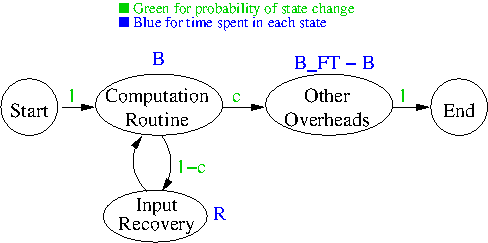
\includegraphics[width=8cm,natwidth=488,natheight=243]{model1.png}
\label{markovModel}
\caption{Markov Model used for modeling running time under low error rates.}
\end{figure}

\section{Conclusion}

As far as the scope of this report is concerned, we have extended our experiments from the Lasso application in the DSN paper to another two applications, DRC and Hattrick (By the time the report is submitted, Hattrick is still in progress). We have also taken the step into exploring the configuration space of error checker thresholds and have found there should exist an optimal threshold choice that varies according to experiment configurations. We have devised two metrics, the accuracy metric and the running time metric, to quantify the effectiveness of our fault-tolerance mechanisms.


\nocite{5764677}
\nocite{Rinard:2006:PAB:1183401.1183447}
\nocite{deKruijf:2010:RAF:1816038.1816026}
\nocite{deKruijf:2010:RAF:1815961.1816026}
\nocite{Riesen:2011:SAR:2238436.2238466}
\nocite{1386657}
\nocite{journals/ijhpca/CappelloGGKKS09}
\nocite{Restrepo-Calle:2010:CIF:1811212.1811218}
\nocite{6264672}
\nocite{deKruijf:2011:IPA:2155620.2155637}
\nocite{Baek10green:a}
\nocite{Hoffmann:2011:DKR:1961295.1950390}
\nocite{Chan:2009:AMP:1654059.1654065}
\nocite{Cui:2012:EPO:2355585.2355587}
\nocite{1402092}
\nocite{deKruijf:2012:SAC:2345156.2254120}
\nocite{Abadi:2009:CIP:1609956.1609960}
\nocite{Reis:2005:SFT:1113841.1113843}
\nocite{lee2011sef}
\nocite{6012845}

%%%%%%%%%%%%%%%%%%%%%%%%%%%%%%%%%%%%

%\appendix
%\section{Appendix Title}

%This is the text of the appendix, if you need one.

%\acks

%Acknowledgments, if needed.

% We recommend abbrvnat bibliography style.


%\bibliographystyle{abbrvnat}
\bibliographystyle{plain}
% The bibliography should be embedded for final submission.


\bibliography{./bibs}


\end{document}
